\label{sec:experiment}

\begin{figure*}[t]
  \begin{minipage}[t]{0.32\linewidth}  
  \centering
  \subfigure[NetVLAD/1frame.] {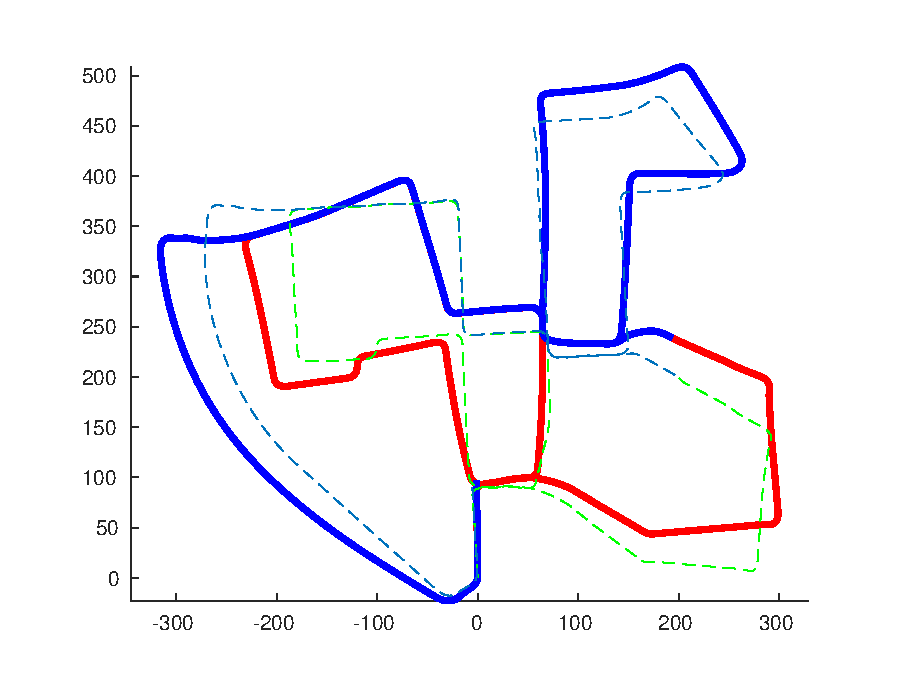
\includegraphics[width=0.75\linewidth]{fig/1netvlad.eps}\label{fig:1netvlad}}
  \end{minipage}
  \begin{minipage}[t]{0.32\linewidth}  
  \centering  
  \subfigure[NetVLAD/4frames.] {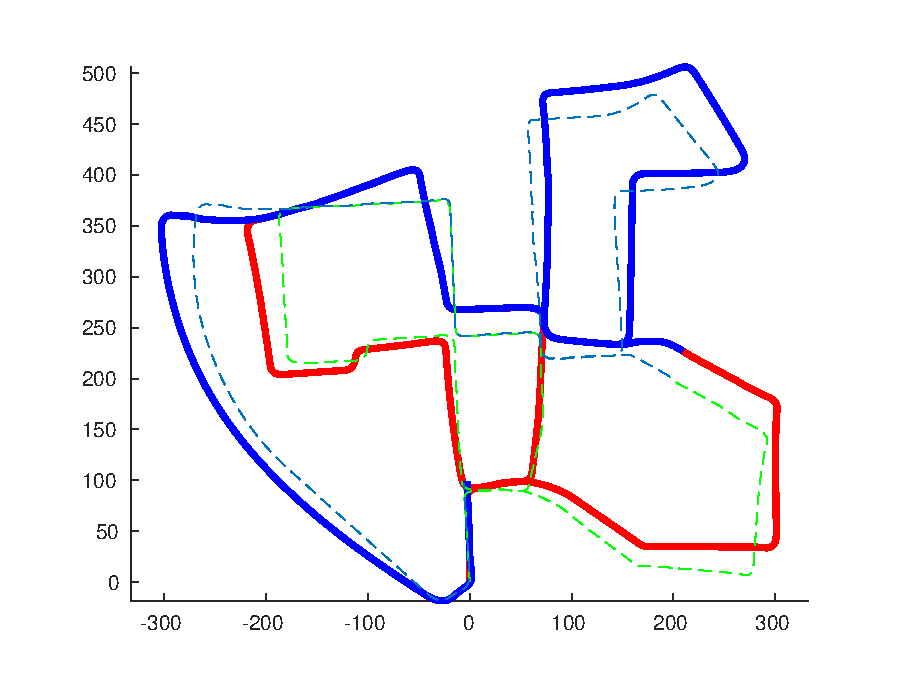
\includegraphics[width=0.75\linewidth]{fig/4netvlad.eps}\label{fig:4netvlad}} 
  \end{minipage}
  \begin{minipage}[t]{0.32\linewidth}  
  \centering  
  \subfigure[NetVLAD/8frames.] {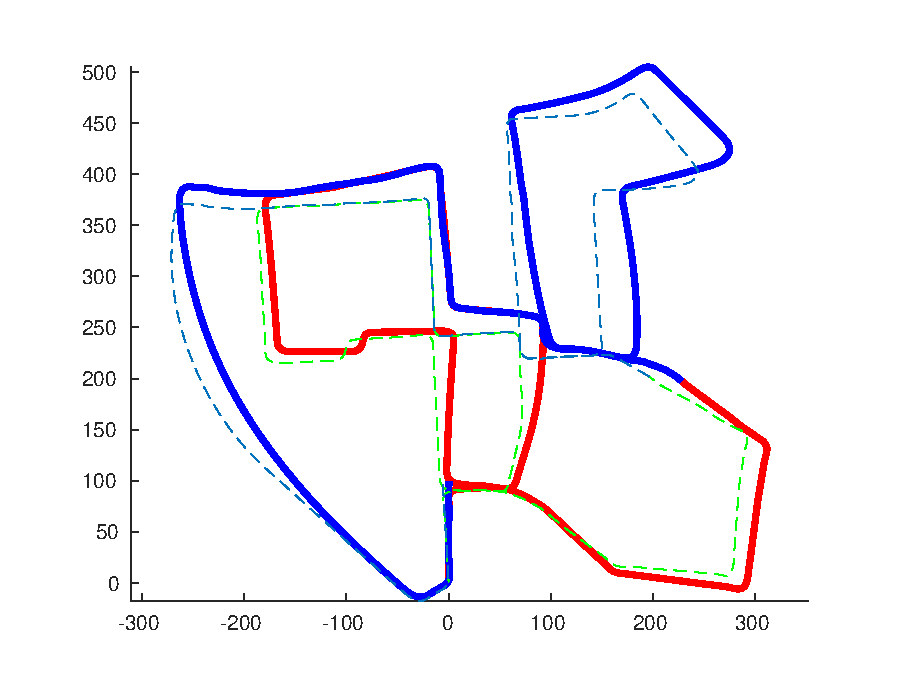
\includegraphics[width=0.75\linewidth]{fig/8netvlad.eps}\label{fig:8netvlad}} 
  \end{minipage}
  
  \begin{minipage}[t]{0.32\linewidth}  
  \centering  
  \subfigure[NetVLAD/10frames.] {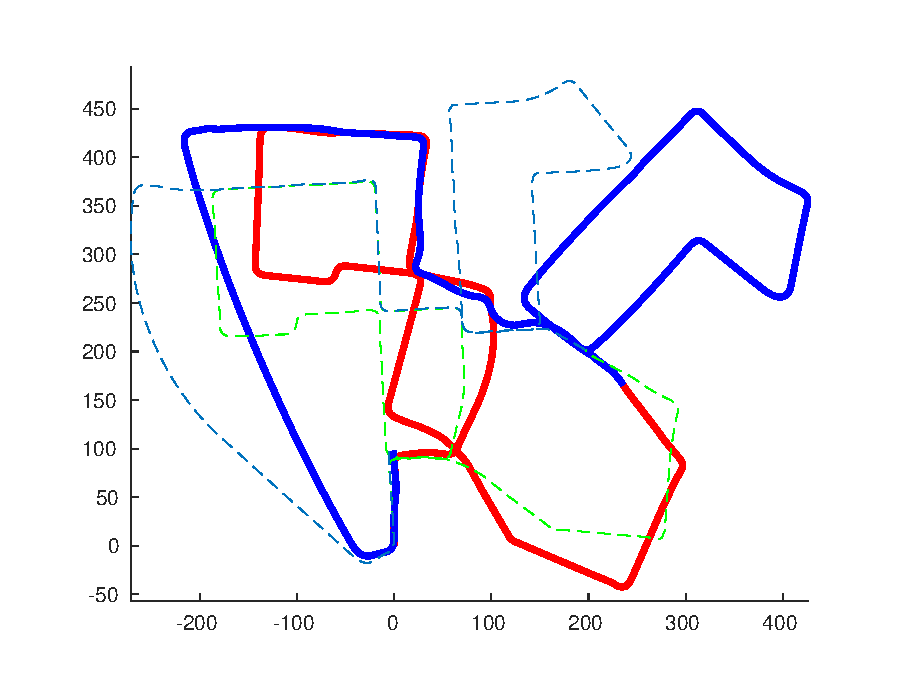
\includegraphics[width=0.75\linewidth]{fig/10netvlad.eps}\label{fig:10netvlad}} 
  \end{minipage}
  \begin{minipage}[t]{0.32\linewidth}  
  \centering  
  \subfigure[NetVLAD/12frames.] {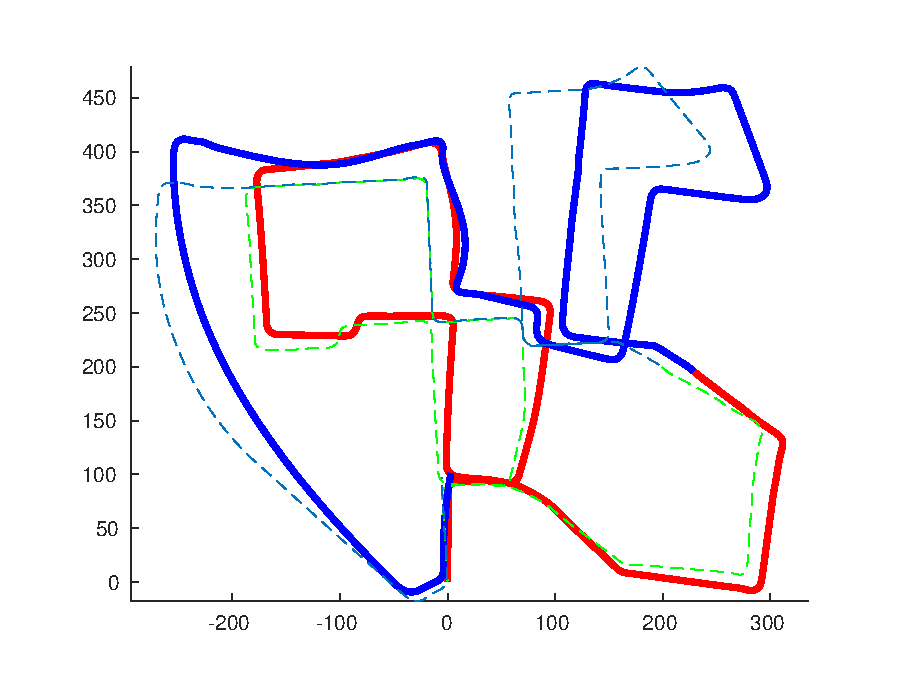
\includegraphics[width=0.75\linewidth]{fig/12netvlad.eps}\label{fig:12netvlad}} 
  \end{minipage}
  \begin{minipage}[t]{0.32\linewidth}  
  \centering  
  \subfigure[NetVLAD/14frames.] {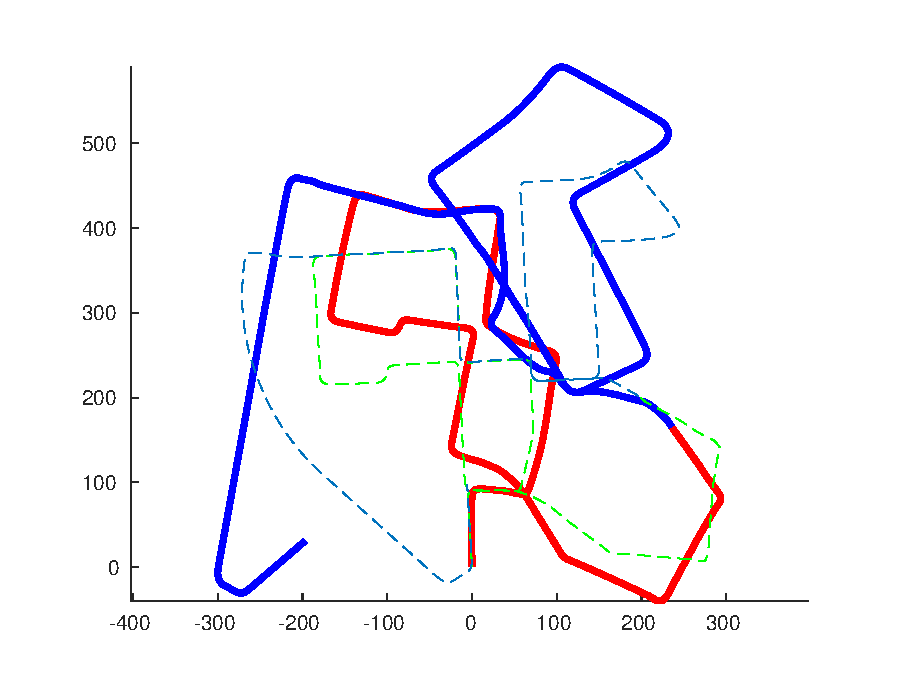
\includegraphics[width=0.75\linewidth]{fig/14netvlad.eps}\label{fig:14netvlad}} 
  \end{minipage}
  \caption{The DSLAM result of two robots(red and blue, the dashed is the ground truth). The higher NetVLAD frequency is, the better the DSLAM performs.
%   (d) find a single intra-robot loop closure which (c) and (d) cannot find, so that the result is better than (c) and (e).
  }
\label{fig:dslamresult}
\end{figure*}

In this section, we will evaluate the speed and accuracy of each proposed CNN components, as well as the impact of our optimization on final DSLAM result.

\subsection{VO with Pose-Sensitive Fixed-Point Finetune}

We evaluate our VO approach with DPU on KITTI dataset \cite{geiger2013vision}. The dataset contains 61 labeled video sequences with stereo pairs, with original image size at $1242 \times 375$ pixels. In the following experiments, we resize the image to $608 \times 160$ in training and testing processes, just like the original Depth-VO-Feat \cite{Zhan:2018e92} does. We use the 00-08 sequences from KITTI as the training set, and evaluate the network on sequence 09 and 10 on the sub-sequences at length of [100,200,...,800] and report the average translational and rotational errors in \cref{tab:VO}. The comparison of the estimated trajectory for different methods is illustrated in \cref{fig:VO}. We use the popular SLAM system, ORB-SLAM \cite{Mur-Artal:2017281}, as the baseline.
 
We use the Pose-Sensitive fixed-point finetune method to balance the speed and accuracy. We use different strategies to split the VONet, and finetune the VONet with the same training superparameters. The initial learning rate is $1e^{-5}$ and the number of finetune iterations is $240000$, which is sufficient to train Depth-VO-Feat from random initialization. We snapshot the network weights every $5000$ iteration, and list the accuracy of the best snapshot in \cref{tab:VO}. The \textit{Quant. Strategy} indicates the configuration of Pose-Sensitive fixed-point finetune. The \textit{Fixed Part} is the feature extraction layers on PL, and the \textit{Float Part} is the pose prediction layers on PS. Because the computation volume of FC layers is much less than that of CONV layers, we can split all of the FC layers into pose prediction network, significantly improving the accuracy by consuming little extra time.



% Because of the fixed-point number used in our design, which sacrifices the precision of the CNN, the VO accuracy is not as good as the previous works \cite{Mur-Artal:2017281, Zhan:2018e92}. On the other hand, our VO can calculate the 6-D pose within $20ms$ on a resource-constrained embedded platform.


\subsection{Run-Time with/without Cross-Module Scheduling}

We evaluate our VO and NetVLAD implementation simutaneously on a Xilinx ZU9 MPSOC. \Cref{tab:time} shows the run time of each part of our DSLAM system.


% \begin{figure}[t]
%     \centering  
%     \includegraphics[width=0.95\linewidth]{fig/env.eps}
%     \caption{The intelligent car with the Zynq MPSoC board.}
%     \label{fig:env}
% \end{figure}

\begin{table}[h]
    \centering
    \caption{Run time of each part in our DSLAM}
    \footnotesize
    \begin{threeparttable}
  % Table generated by Excel2LaTeX from sheet 'Sheet2'
  \setlength{\tabcolsep}{1mm}{
% Table generated by Excel2LaTeX from sheet 'Sheet1'
\begin{tabular}{|c|c|c|c|c|c|c|}
\hline
      & VO    & DPR & DPR, PL & VO, PL  & VO, PS  & DPR, PS  \bigstrut[t]\\
      & ($T_{V}$) & ($T_{D}$) & ($T_{0}$) &  ($T_{1}$) &  ($T_{2}$) &  ($T_{3}$) \bigstrut[b]\\
\hline
Execute & \multirow{2}[2]{*}{13} & \multirow{2}[2]{*}{422} & \multirow{2}[2]{*}{66} & \multirow{2}[2]{*}{3} & \multirow{2}[2]{*}{10} & \multirow{2}[2]{*}{356} \bigstrut[t]\\
 time (ms)  &       &       &       &       &       &  \bigstrut[b]\\
\hline
\end{tabular}%

    
  }
  \begin{tablenotes}
        \item[*] We read the camera at 20fps, so the $T_{f}$ in \cref{fig:pipline} is 50ms.
        \item[*] We use the NetVLAD method to do DPR in this paper.
        \end{tablenotes}
      \end{threeparttable}
    \label{tab:time}%
    
  \end{table}%

Since the NetVLAD frequency ($N$) before cross-module scheduling is constrained by \cref{equ:serial}, NetVLAD can be calculated once every 12 frames. We divide the running time of the DSLAM into three threads: PL, VO on PS, NetVLAD on PS, and we calculate the running time of each part, which satisfies \cref{equ:pipeline1,equ:pipeline2,equ:pipeline3} respectively. Then we find out that run-time of the NetVLAD on PS ($T_{3}$) is the bottleneck of DSLAM system and \cref{equ:pipeline3} constrains the NetVLAD frequency ($N$) to $8$.

%Substituting the run-time of each part into \cref{equ:pipeline1,equ:pipeline2,equ:pipeline3}, we find out that run-time of the NetVLAD on PS ($T_{3}$) becomes the bottleneck of the system and \cref{equ:pipeline3} constrains the NetVLAD frequency ($N$) to $8$.

The effect of NetVLAD frequency on the DSLAM result will be further discussed in \cref{sec:dlamexp}.  

\subsection{NetVLAD with DPU}

We evaluate the NetVLAD performance on the loop-closure dataset based on KITTI \cite{KITTIGroundTruth}.
The dataset labels the ground truth of loop closure for these sequences based on the metric positions of each image. Specifically, it compares the position of each image to the others in the sequence and regards the one as a loop if it lies within a radius of $6m$.

The precision-recall curves of the original NetVLAD with an output of 4096 dimensions (Blue), fixed-point NetVLAD 4096-D output (Green), original NetVLAD with 128-D output (Red), and fixed-point NetVLAD 128-D output (Yellow) are shown in \cref{fig:reloc}. We take sequence 00 as the test sequence, and achieve similar accuracy with the floating-point model of the same output dimensions.


\begin{figure}[thb]
  \centering  
  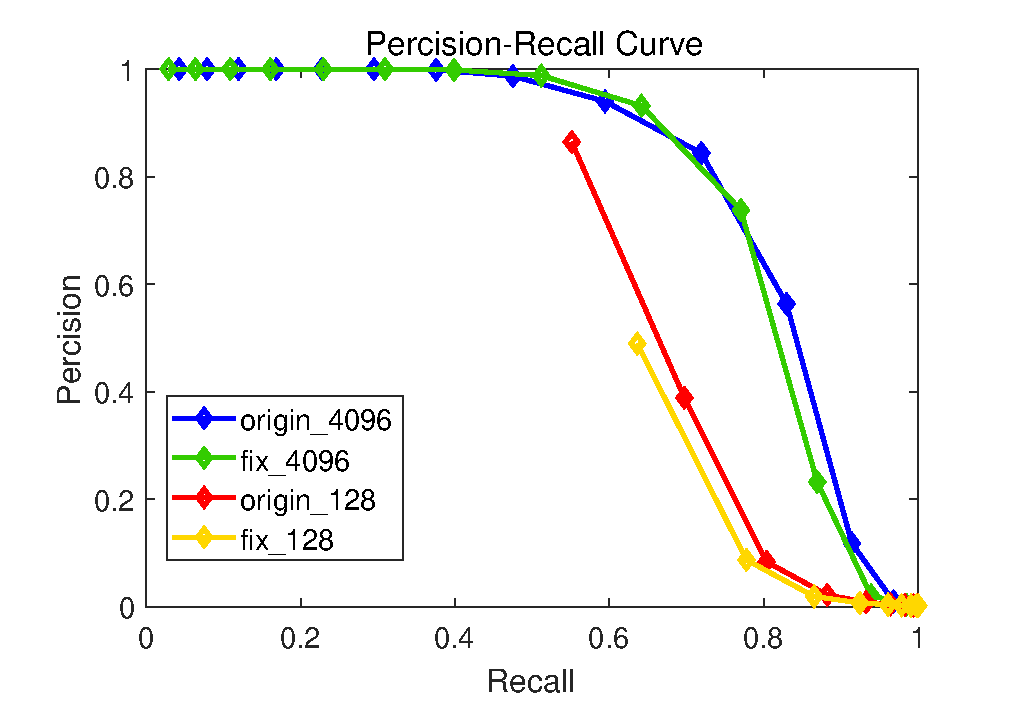
\includegraphics[width=0.95\linewidth]{fig/val_reloc.eps}
  \caption{ROC curves on sequence 00.}
  \label{fig:reloc}
\end{figure}

\subsection{DSLAM Evaluation}
\label{sec:dlamexp}

\begin{figure}[thb]
  \centering  
  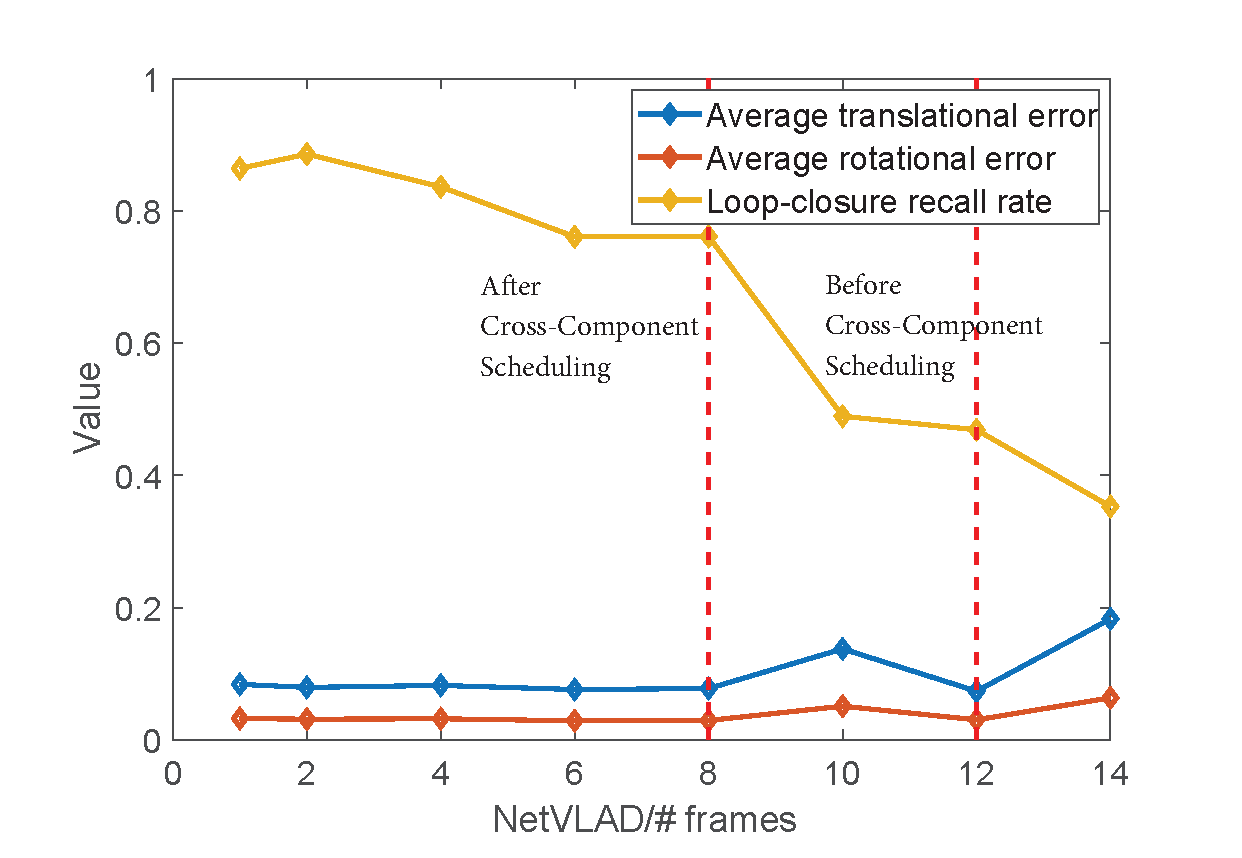
\includegraphics[width=0.95\linewidth]{fig/dslam_curve.eps}
  \caption{ATE, ARE and LCR curves on sequence 00. For ATE and ARE, lower is better, and for LCR, higher is better. Lower $NetVLAD /\sharp frames$  means higher NetVLAD frequency. The NetVLAD frequency is $NetVLAD/12frames$ for serial scheduling and  $NetVLAD/8frames$ for Cross-Component scheduling.}
  \label{fig:curves}
\end{figure}


We evaluate our DSLAM system on KITTI odometry dataset. Firstly we divide the KITTI sequence into 2 subsequences with a 10-frame overlap, and resize the input image to  $608 \times 160$ for VO and DPR. We treat each subsequence as the raw data for each robot. 

We use the same method in \cite{Cieslewski:20187ee} to simulate the DOpt and merge the two trajectories. The DOpt method used in this work is proposed in \cite{Choudhary:2017e66}.
% , which is a two-stage approach to solve the optimization problem in a decentralized manner: 1) First, it gets an estimation for the rotations of all robots, and 2) then it recovers the full poses and top-off the result with a Gauss-Newton (GN) iteration.

We run each subsequence on the Xilinx MPSoC ZU9 platform to get the results of VO and DPR. The merged trajectories before and after cross-module scheduling are shown in \cref{fig:12netvlad,fig:8netvlad}. The results of other  NetVLAD frequencies, illustrated as \cref{fig:1netvlad,fig:10netvlad,fig:12netvlad}, are simulated with the fixed-point CNN model on desktop computer.

% To further explore the effect of NetVLAD frequency on the final DSLAM result, we run the fixed-point NetVLAD model with different frequency on our desktop computer, and do DOpt with the same VO results from Xilinx MPSoC ZU9. More merged trajectories with different NetVLAD frequency are illustrated as \cref{fig:1netvlad,fig:10netvlad,fig:12netvlad}.

Tranditional indicators, such as average translational error (ATE) and average rotational error(ARE), can not demonstrate the performance of trajectory merging in DSLAM, so we propose a new metric called loop-closure recall rate (LCR) to evaluate the DSLAM system. LCR indicates the success rate of loop-closure detection on the merged trajectory, which can reflect the performance of trajectory merging. LCR is calculated by the following formula:$$LCR=\frac{\eta_{merged\ tracjectory}}{\eta_{groundtruth}}$$, where $\eta$ is the number of frame pairs with successful place recognition. In our experiments, when the Euclidean distance between one point  and the other point on the trajectory is less than 6 meters, just like \cite{zhang2018graph}, we think that this is the place that has been reached before, that is, the location matches, forming a loop.

\Cref{fig:curves} shows that with the increase of the NetVLAD frequency, there is a downward trend on ATE and ARE. However, the ATE and ARE strongly depend on the loop-closure result, and a single accidentally detected loop-closure will dramatically change the trajectory. That's why \cref{fig:12netvlad} performers better than \cref{fig:10netvlad} with a lower NetVLAD frequency. The LCR can efficiently indicate the trajectory merging performance: as the NetVLAD frequency increases, the LCR curve also increases.

From \cref{fig:dslamresult} and \cref{fig:curves}, we can conclude that the NetVLAD frequency higher than $NetVLAD/8frames$  reach a similar high level performance in different indicators. Continuous improvement of the NetVLAD frequency from $NetVLAD/8frames$ has limited effect on the final DSLAM performance. Our cross-component scheduling method can improve the NetVLAD frequency from  $NetVLAD/12frames$ to  $NetVLAD/8frames$, and thus significantly evolve the DSLAM performance.